\documentclass{article}
\usepackage[utf8]{inputenc}
\usepackage{caption}
\usepackage{amsmath}
\usepackage{amssymb}
\usepackage{mathtools}
\usepackage{multicol}
\usepackage{graphicx}
\usepackage{wrapfig}
\usepackage{float}
\usepackage[makeroom]{cancel}

\graphicspath{ {./images/} }

\renewcommand{\baselinestretch}{1.5} % line spacing
\newcommand{\fline}{\par\noindent\rule{\textwidth}{0.1pt}} % horizontal line (wide)

\title{Dynamics Lab\\Acceleration with a Pulley}
\author{Peter Zhang}

\begin{document}

\maketitle
\newpage
\tableofcontents
\newpage


\section{Purpose}
To compare the experimental acceleration to the theoretical acceleration for an object moving horizontally while being pulled by a hanging mass.

\section{Data Tables}

\begin{center}
	\begin{tabular}{|c|c|}
		\hline
		Variable & Measured Value\\
		\hline \hline
		$m_{car}$ & $545.7g\pm1g$\\
		\hline
		$m_{weight\ 1}$ & $20g\pm0.2g$\\
		\hline
		$m_{weight\ 2}$ & $50g\pm0.2g$\\
		\hline
	\end{tabular}
	\captionof{table}{Measured Values}
\end{center}

\begin{center}
	\begin{tabular}{|c|c|}
		\hline
		Variable & Value\\
		\hline \hline
		$v_{i}$ & $0m/s$\\
		\hline
		$g$ & $9.8m/s^2$\\
		\hline
		$f$ (friction) & assume none $\therefore{0}$\\
		\hline
	\end{tabular}
	\captionof{table}{Other Values}
\end{center}

\begin{center}
	\begin{tabular}{|c|c|}
		\hline
		Variable & Calculated Value\\
		\hline \hline
		$m_{t}$ & $m_{weight\ 1} + m_{weight\ 2} = 70g\pm0.4g$\\
		\hline
		$a_{car}$ (calculated with LoggerPro) & $1.100\pm0.1160m/s$\\
		\hline
	\end{tabular}
	\captionof{table}{Calculated Values}
\end{center}

\begin{figure}[H]
	\centering
	\fbox{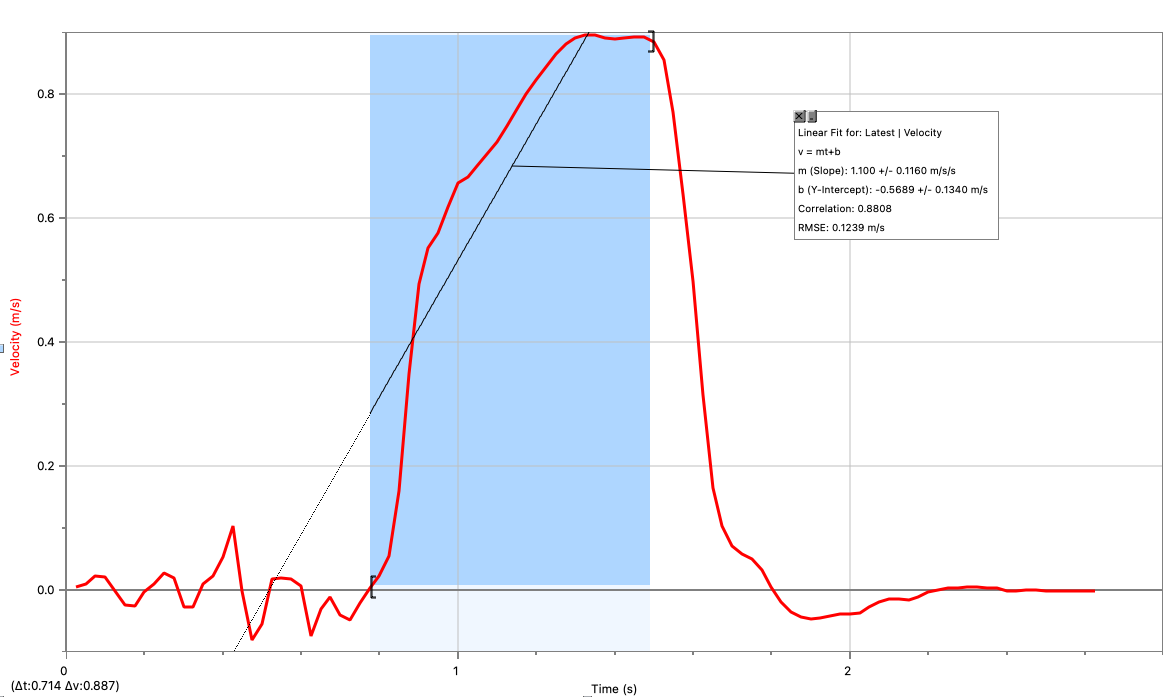
\includegraphics[width=\textwidth]{graph_line_x.png}}
	\captionof{figure}{Velocity Time Graph with Line of Best Fit}
\end{figure}

\begin{figure}[H]
	\centering
	\fbox{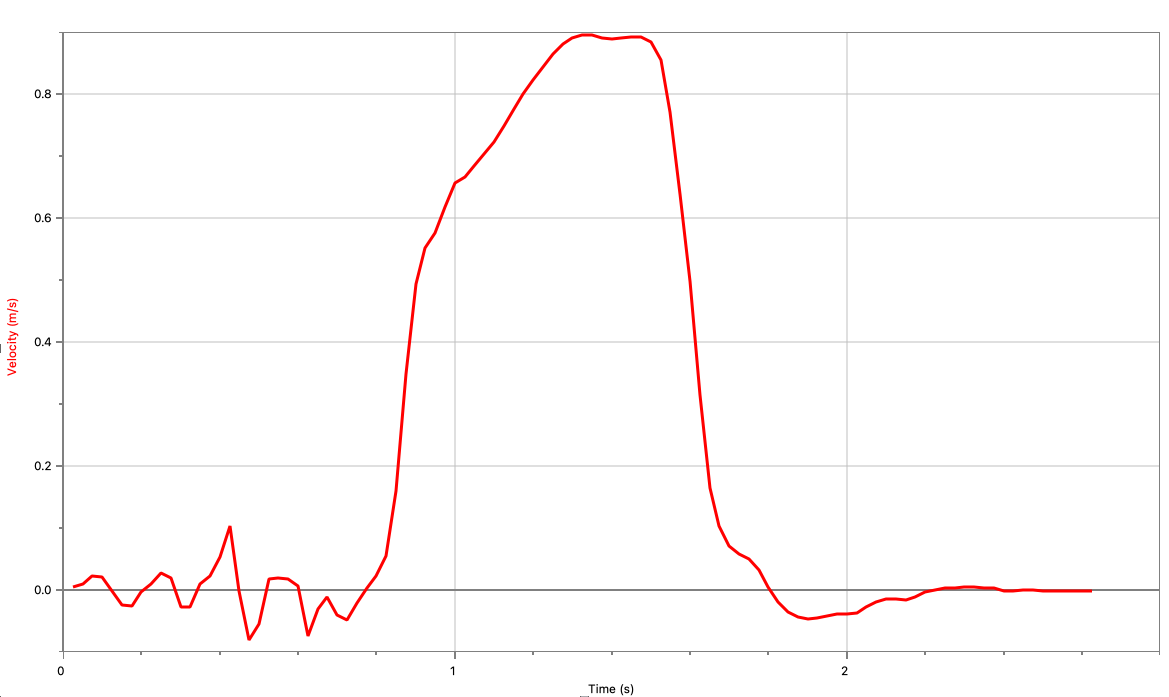
\includegraphics[width=\textwidth]{graph_no_line.png}}
	\captionof{figure}{Velocity Time Graph without Line of Best Fit}
\end{figure}






\section{Analysis}

\begin{figure}[H]
	\centering
	\fbox{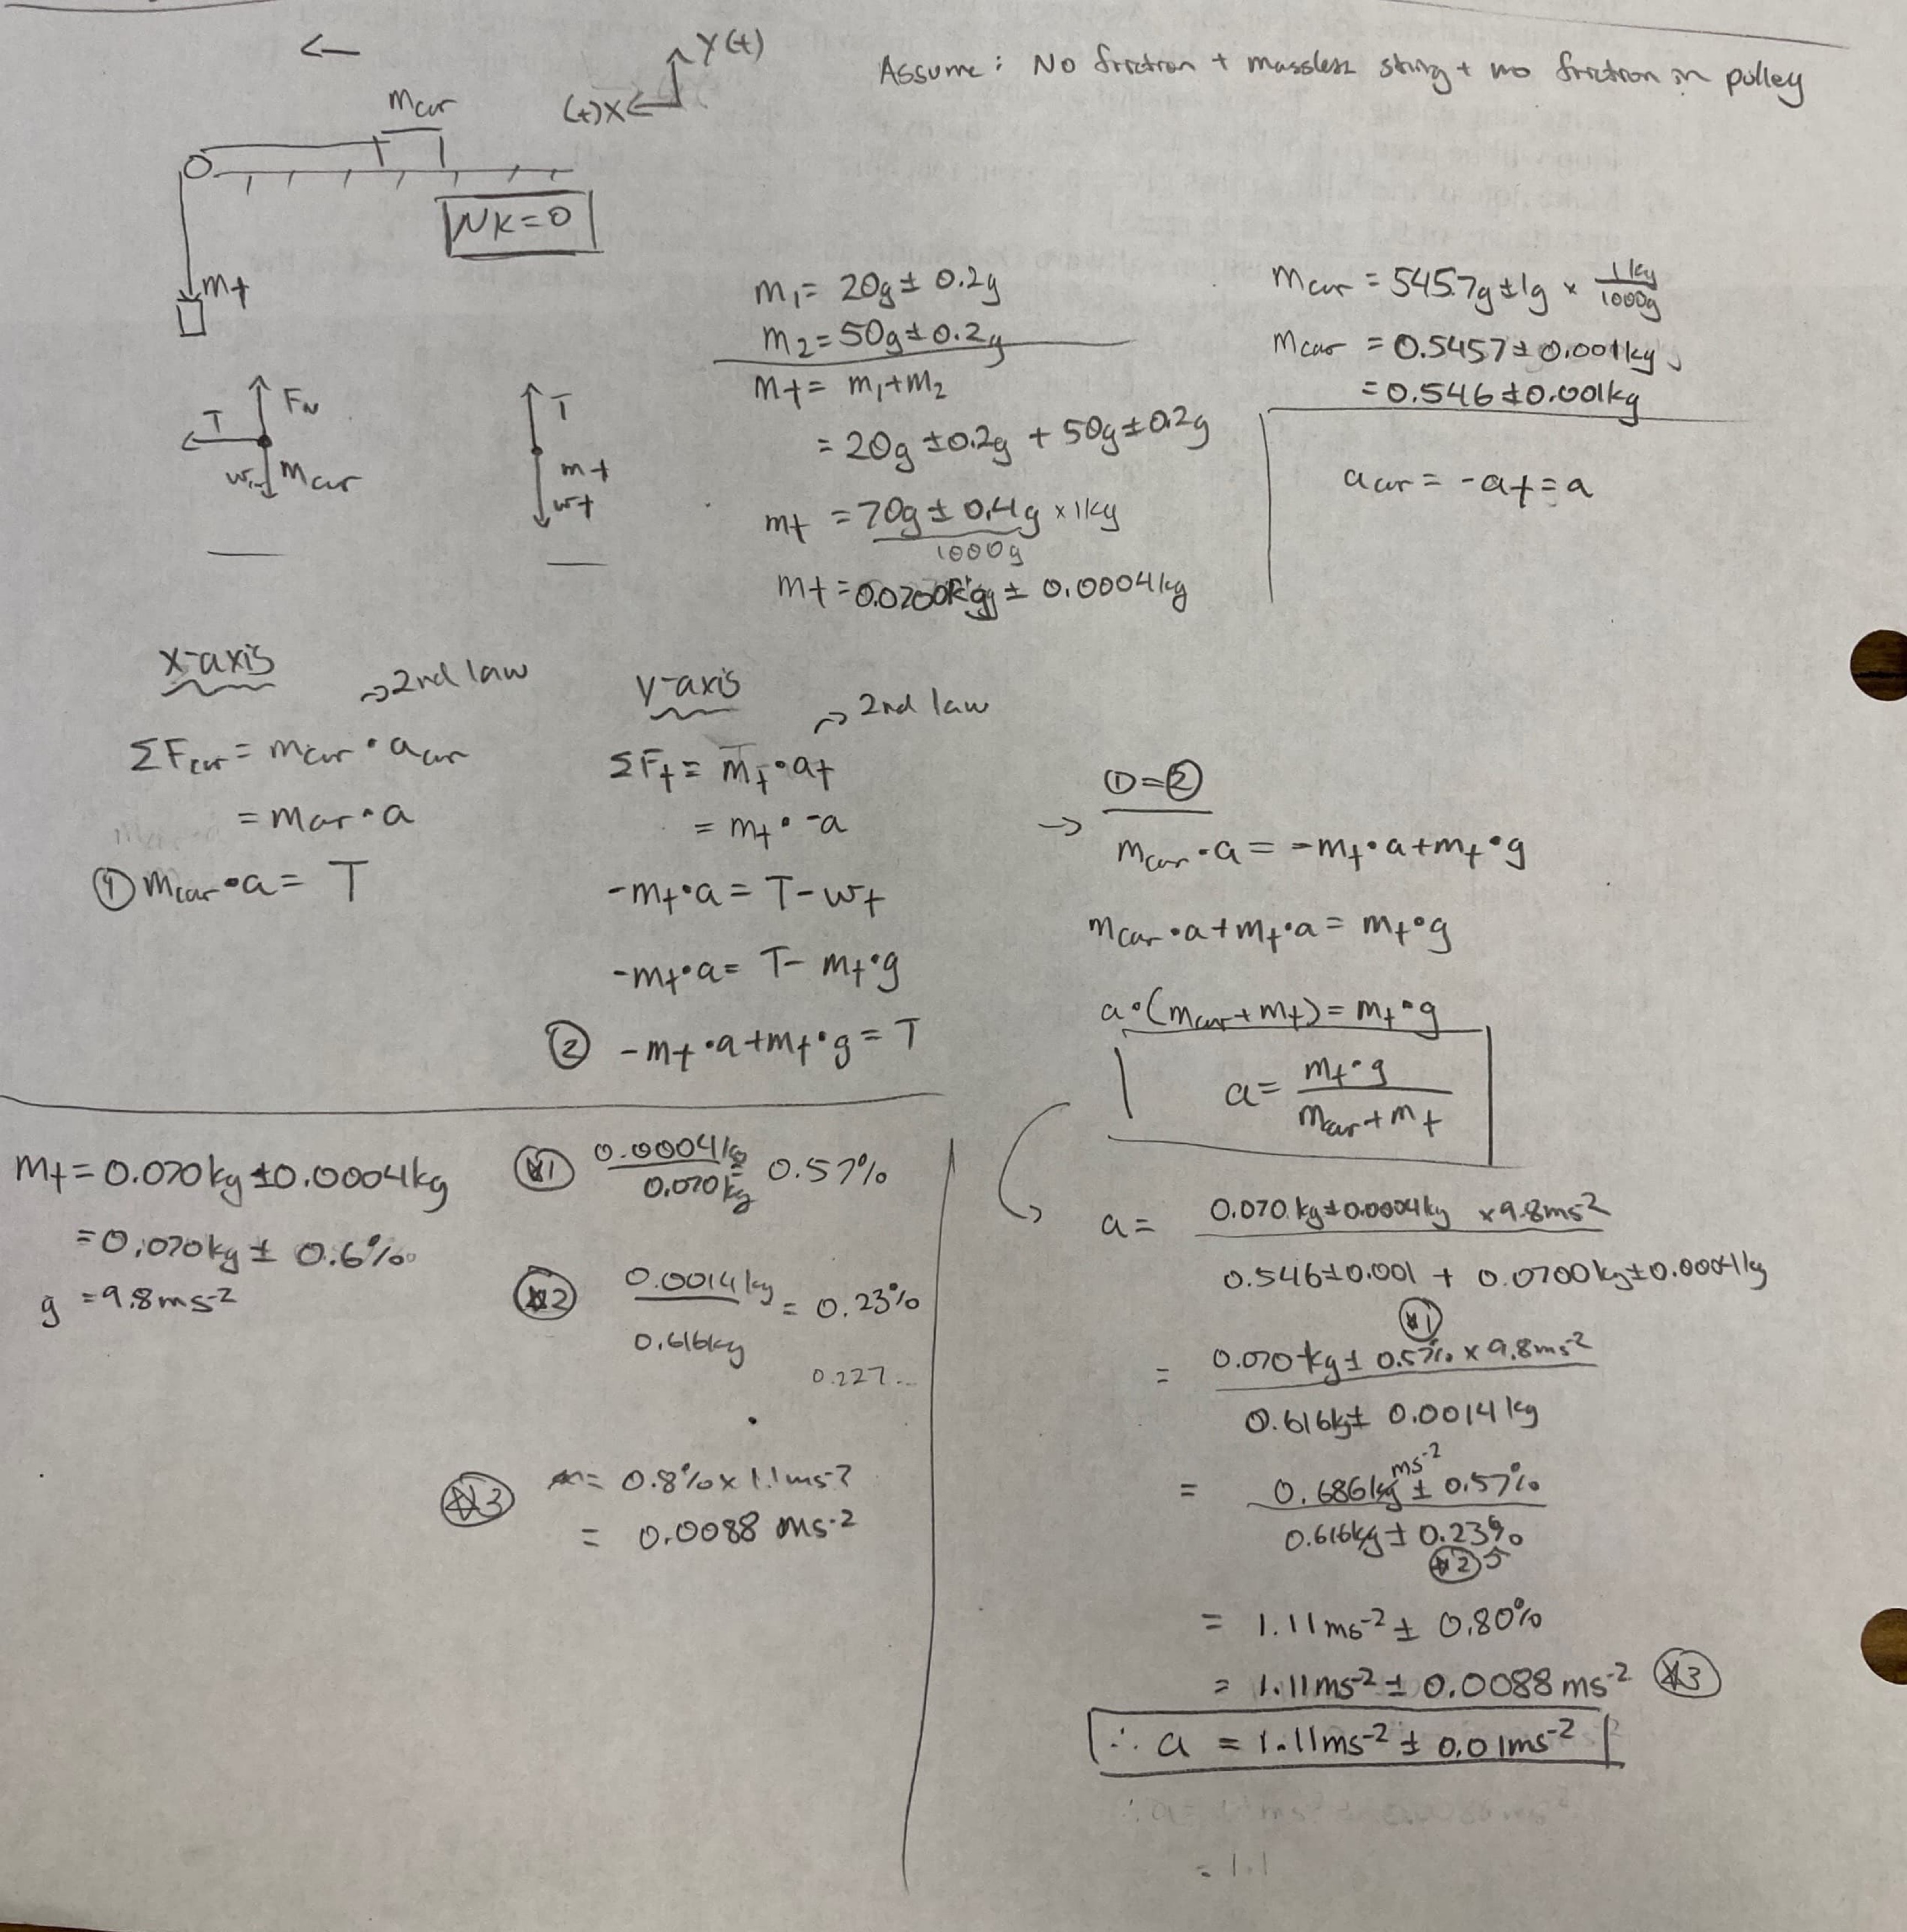
\includegraphics[width=\textwidth]{calculations.JPG}}
	\captionof{figure}{Calculations}
\end{figure}

\subsection{Assumptions}
\begin{itemize}
\item no friction
\item massless string
\item massless pulley
\item no frictino in pulley
\end{itemize}

\pagebreak

\subsection{Question 1}
Derive using Newton's Laws, the expected accleration as a function of the mass of the cart ($m_{c}$) and the falling mass ($m_{t}$)

\begin{figure}[H]
	\fbox{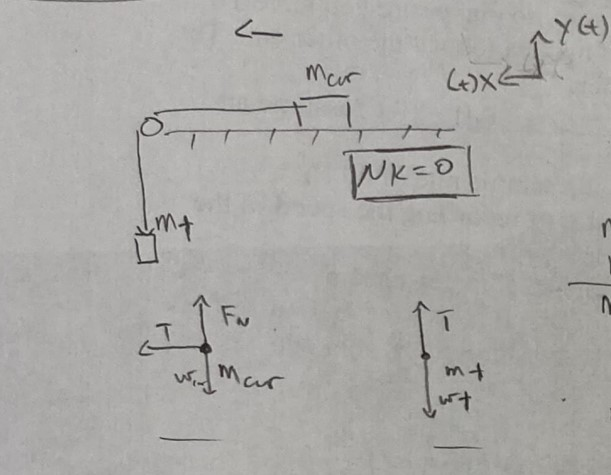
\includegraphics[width=\textwidth]{diagram.png}}
	\captionof{figure}{Diagram of System \& Free Body Diagrams}
\end{figure}

Set acceleration according to direction of motion in diagram
\begin{center}
$a_{car} = -a_{t} = a$
\end{center}

\subsubsection{x-axis (car)}
\begin{align*}
\sum{F_{car}} 		& = m_{car} * a_{car}	(2nd law) \\
\therefore 			& m_{car} * a \\
[1] m_{car} * a 			& = T
\end{align*}

\subsubsection{y-axis (weight)}
\begin{align*}
\sum{F_{t}} 		& = m_{t} * a_{t}	(2nd law) \\
				& = m_{t} * (-a) \\
-m_{t}*a 		& = T - w_{t} \\
-m_{t}*a 		& = T - m_{t}*g \\
[2] -m_{t}*a + m_{t}* g		& = T
\end{align*}


\subsubsection{\underline{[1] = [2]}}
\begin{align*}
[1] & = [2] (since T_{car} = T_{weight}) \\
m_{car}*a 		& = -m_{t}*a + m_{t}*g \\
m_{car}*a + m_{t}*a 	& = m_{t}*g \\
a*[m_{car} + m_{t}] 	& = m_{t}*g \\
\Aboxed{a & = \frac{m_{t}*g}{m_{car} + m_{t}}}
\end{align*}

\pagebreak

\subsection{Question 2}
Using the values for the mass of the car and the falling mass, determine the value of your expected acceleration.

Convert mass from grams to kilograms
\begin{align*}
m_{t} 		& = (70g\pm0.4g) * \frac{1kg}{1000g}\\
			& = 0.0700kg\pm0.0004kg\\
\\
m_{car}		& = (545.7g\pm1g) * \frac{1kg}{1000g}\\
			& = 0.5457\pm0.0001kg
\end{align*}

Plug in values with uncertainties and solve for $a$
\begin{align*}
a 			& = \frac{(0.0700\pm0.0004kg) * 9.8m/s^2}{(0.546\pm0.001kg) + (0.0700\pm0.0004kg)}\\
a 			& = \frac{(0.0700\pm0.57...\%) * 9.8m/s^2}{(0.546\pm0.001kg) + (0.0700\pm0.0004kg)}\\
a 			& = \frac{(0.0700\pm0.57...\%) * 9.8m/s^2}{0.616\pm0.0014kg}\\
a 			& = \frac{0.686kgm/s^2\pm0.57...\%}{0.616kg\pm0.0014kg}\\
a 			& = \frac{0.686kgm/s^2\pm0.57...\%}{0.616kg\pm0.23...\%}\\
a 			& = 1.11m/s^2 \pm 0.80...\%\\
a 			& = 1.11m/s^2 \pm 0.0088m/s^2\\
\Aboxed{a 	& = 1.11m/s^2 \pm 0.01m/s^2}
\end{align*}

\pagebreak

\subsection{Question 3}
Make a data/results table

\begin{center}
	\begin{tabular}{|c|c|}
		\hline
		Variable & Result\\
		\hline \hline
		Experimental Acceleration & $0.61m/s^2\pm0.05m/s^2$\\
		\hline
		Expected Acceleration & $1.11m/s^2 \pm 0.01m/s^2$\\
		\hline
	\end{tabular}
	\captionof{table}{Data/Results Table}
\end{center}

\pagebreak

\section{Discussion}

\subsection{Question1}
Does your experimental acceleration agree within uncertainty with your expected acceleration?

\begin{align*}
Taken from previous question\\
a_{max}		& = 1.11m/s^2 + 0.01m/s^2\\
a_{max} 	& = 1.12m/s^2\\
\\
a_{min}		& = 1.11m/s^2 - 0.01m/s^2\\
a_{min}		& = 1.10m/s^2
\\
a_{experimental} = 1.100\pm0.1160m/s\\
\therefore a_{min}\leq a_{experimental}\leq  a_{max}
\end{align*}

The experimental acceleration agrees with the uncertainty of the lab.


\subsection{Question 2}
State at least 3 relevant and significant sources of error in this lab.





\end{document}
